

%!TEX root = ../Notes.tex
\chapter{Definitions and Examples} 
\section{Introduction} \textbf{ What is geometry?} Geometry is the study of rigid shapes that can be distinguished with measurements (length, angle, area, \ldots).

\textbf{ What is topology?} Topology is the study of shapes which are equivalent via deformations. 

\textbf{ Topology versus Geometry:} Objects that have the same topology do not necessarily have the same geometry. For instance, a square and a triangle have different geometries but the same topology.

% I'm going to use the \[\includegraphics[]{}\] syntax for most of the pictures.
% This is because I really do want them in very specific places, and LaTeX enjoys
% moving figures around even when I tell it not to do so.
\[ 
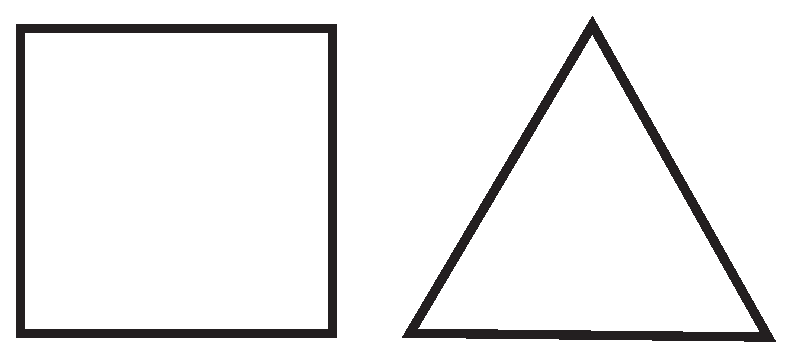
\includegraphics[width=150pt]{images/intro_and_review/square_and_triangle} \]

\textbf{ Motivation:} Our goal is to understand the shape of our universe. Consider the following examples of two-dimensional universes: a plane, a sphere, a torus, and planes connected by tubes.
\[ 
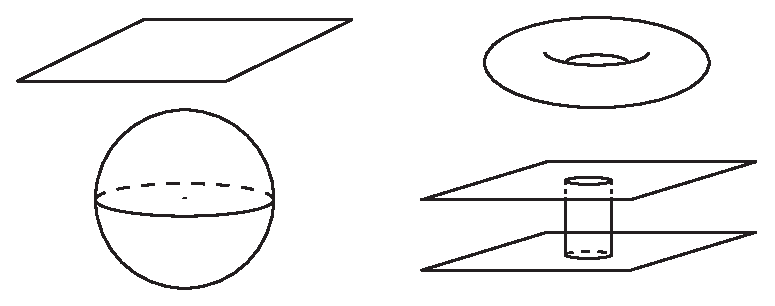
\includegraphics[width=300pt]{images/intro_and_review/various_shapes} \]

\noindent These are topologically distinct universes. Intuitively, we can see that their ``holes'' distinguish them. Hence we seek a mathematical way to describe the holes; one familiar concept we will use is continuity, which is related to a lack of holes.

\section{Some Review from Analysis} 
\begin{definition}
	Let $f : \R \rightarrow \R$ and $a \in \R$. We say $f$ is \textbf{continuous} at $a$ if $\forall \epsilon > 0$ $\exists$ $\delta > 0$ such that if $|x-a|<\delta$, then $|f(x)-f(a)|<\epsilon$. 
\end{definition}
\begin{definition}
	Let $M$ be a set and $d: M \times M \rightarrow \R$ be a function such that 
	\begin{enumerate}
		\item $d(a,b)=0$ iff $a=b$ (\textbf{nondegeneracy}) 
		\item $\forall a,b,c \in M$, $d(b,c) \leq d(a,b) + d(a,c)$ (\textbf{triangle inequality}). 
	\end{enumerate}
	Then we say $d$ is a \textbf{metric} or distance and $(M,d)$ denotes a \textbf{metric space}. 
\end{definition}

\noindent Compare this to the usual definition of a metric space. The above definition is equivalent to the usual definition of a metric space, but does not explicitly state the properties of positivity or symmetry: 
\begin{enumerate}
	\item $d(a,b) \geq 0$ $\forall a,b \in M$ (\textbf{positivity}) 
	\item $d(a,b) = d(b,a)$ $\forall a,b \in M$ (\textbf{symmetry}). 
\end{enumerate}
\begin{definition}
	The \textbf{usual metric} on $\R^{n}$ is
	\[ d((x_1,\ldots,x_n),(y_1,\ldots,y_n)) = \sqrt{\sum_{i=1}^n (x_i-y_i)^2}. \]
\end{definition}
\begin{definition}
	Let $M$ be any set. Then the \textbf{discrete metric} is defined as
	\[ d(a,b) = \left\{ 
	\begin{array}{lr}
		1 & \text{if } a \neq b \\
		0 & \text{if } a = b 
	\end{array}
	\right. \]
\end{definition}
The discrete metric can be useful for testing conjectures as it does not rely on $\R^n$.
\begin{example}
	[The Comb Metric for $\R^2$.]
	
	Let $X_0 = \{ 0 \} \times [0,1]$, $Y_0 = [0,1] \times \{ 0 \}$; and $\forall n \in \N$, let $X_n = \{ \frac{1}{n} \} \times [0,1]$. Let $M = (\cup_{n=0}^\infty X_n) \cup Y_0$. The distance is the distance measured along the comb in $\R^2$.
	\[ 
	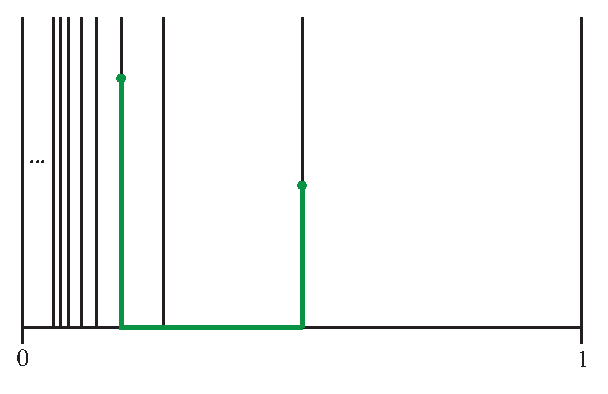
\includegraphics[width=240pt]{images/intro_and_review/comb_space} \]
\end{example}

Using the comb metric, 
\begin{itemize}
	\item Does the sequence $\{ (\frac{1}{n},0) \}$ converge? Yes, to the origin. 
	\item Does the sequence $\{ (\frac{1}{n},a) \}$ converge when $a \in (0,1]$? No, since $d((\frac{1}{n},a),(0,a)) > 2a$ $\forall n$. 
\end{itemize}
\begin{example}
	[A Non-Example of a Metric Space.] Consider the line of real numbers with $d(a,b) = a-b$. Clearly, $d(a,b)=0$ only when $a=b$, satisfying the first property (nondegeneracy). However, the second property (triangle inequality) is not satisfied: if $a=0$, $b=1$, and $c=-1$, then
	\[2=d(b,c) \nleq d(a,b)+d(a,c)=-1+1=0.\]
	Notice that this non-example also fails to satisfy the other two properties listed in the usual definition of a metric, positivity and symmetry. 
\end{example}
\begin{example}
	Let $M$ be a set and $d:M\times M\to \R$ a function which satisfies property $2$ but not property $1$ in the definition of a metric space. Then
	\[d(a,b) = 0 \quad \forall a,b \in M\]
	and $M$ has at least 2 points. 
\end{example}
